\documentclass[11pt,a4paper]{article}
\usepackage[russian]{babel}
\usepackage[utf8]{inputenc}
\usepackage{amsmath}
\usepackage{mathtools} 
\usepackage[russian]{babel}
\usepackage{hyperref}
\usepackage{amssymb}
\usepackage{multicol}
\usepackage{bm}
\usepackage{hhline}
\usepackage{array}
\usepackage{multirow}
\usepackage[hcentering, bindingoffset = 10mm, right = 15 mm, left = 15 mm, top=20mm, bottom = 20 mm]{geometry}
\newcounter{prim}
\newenvironment{prim}{%
	\addtocounter{prim}{1}
	\noindent{\\
		\textbf{\noindentПример \arabic{prim}\\}}%
}{}

\DeclareMathOperator{\tr}{\mathop{tr}}
\DeclareMathOperator{\Ker}{\mathop{Ker}}
\DeclareMathOperator{\im}{\mathop{Im}}
\DeclareMathOperator{\const}{\mathop{const}}
\DeclareMathOperator{\rg}{\mathop{rg}}
\newtheorem{definition}{Определение}[section]
\newtheorem{theorem}{Теорема}[section]
\renewcommand{\labelenumi}{\asbuk{enumi})}

\begin{document}
	\part*{Лабораторная работа 3.2.5}
	\part*{Вынужденные колебания в электрическом контуре}
	\textbf{Работу выполнили:} \\
	{\itshape Морозов Матвей \\ Бабушкина Татьяна \\ 678 группа} \\\\
\textbf{Цель работы:} исследование вынужденных колебаний и процессов их установления.
\\\\
\textbf {В работе используются:} генератор звуковой частоты, осциллограф, вольтметр, ёмкость, индуктивность, магазин сопротивлений, универсальный мост.
\\
\part*{Схема установки}
\begin{figure}[h!]
	\centering
	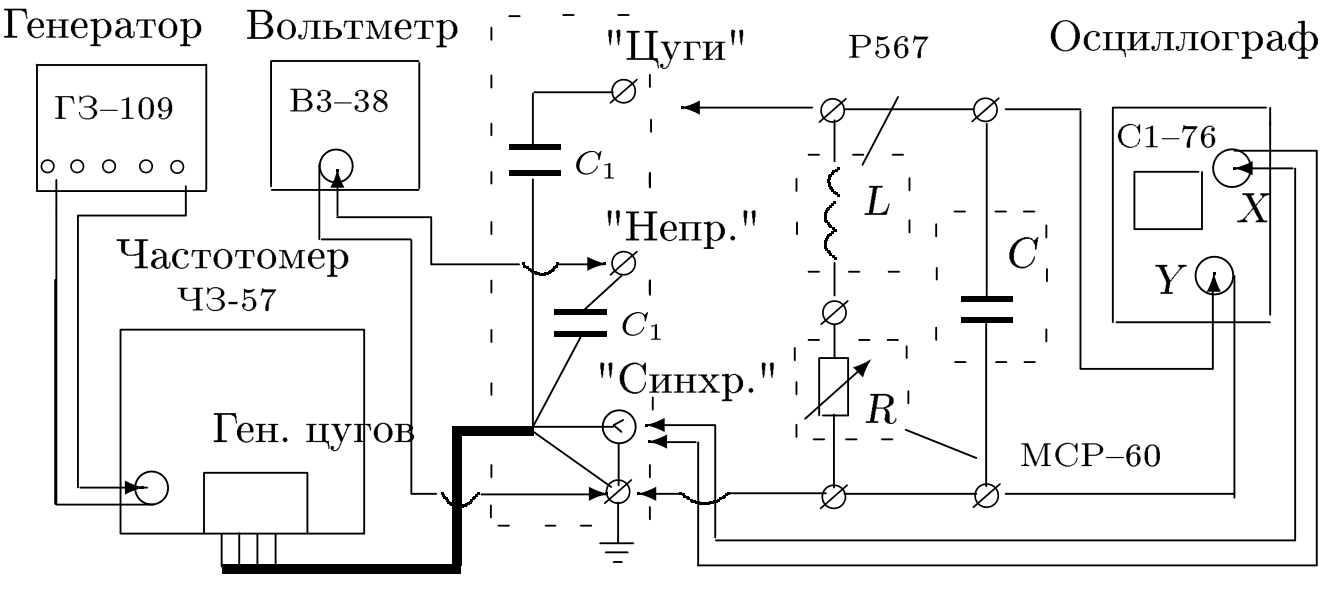
\includegraphics[width=0.8\linewidth]{2}

\end{figure}
\newpage
\part*{Обработка результатов}
\textbf{1)} Изменяя частоту генератора в обе стороны от резонансной, сняли зависимость показаний вольтметра $U$ от показаний частотометра $\nu$. Результаты занесём в таблицу $1$.
	\begin{table}[h!]
	\begin{center}
		\textbf{Таблица 1}. Зависимость $U$ от $f$ при $R=0 \ \ \text{Ом}$.\\
		\begin{tabular}{|c|c|c|c|c|c|c|c|c|c|}
			\hline
№ & $U,\text{мВ}$ & $f,\text{Гц}$ &$U/U_0$ &$f/f_0$ & № & $U,\text{мВ}$ & $f,\text{Гц}$ &$U/U_0$ &$f/f_0$ \\ \hline
$\textbf{1}$ & $0,2$ &	$1278$ &$0,02$ & $0,8023$ & $\textbf{19}$ & $8,2$ & $1583$ & $0,82$ & $0,9937$\\ \hline
$\textbf{2}$ & $0,8$ &	$1396$ &$0,08$ & $0,8763$ & $\textbf{20}$ & $8,8$ & $1585$ & $0,88$ & $0,9950$\\ \hline
$\textbf{3}$ & $1,2$ &	$1449$ & $0,12$ & $0,9096$ & $\textbf{21}$ & $9,2$ & $1589$ & $0,92$ & $0,9975$ \\ \hline
$\textbf{4}$ & $1,6$ &  $1482$ & $0,16$ & $0,9303$ & $\textbf{22}$ & $9,6$ & $1590$ & $0,96$ & $0,9981$\\ \hline
$\textbf{5}$ & $2,0$ &  $1506$  & $0,20$ & $0,9454$ & $\textbf{23}$& $10,0$ & $1593$ & $1,00$ & $1,0000$\\ \hline
$\textbf{6}$ & $2,5$ &	$1520$ & $0,25$ & $0,9542$ & $\textbf{24}$ & $9,2$ & $1607$ & $0,92$ & $1,0088$\\ \hline
$\textbf{7}$ & $3,0$ &	$1530$ & $0,30$ & $0,9605$ & $\textbf{25}$ & $8,8$ & $1609$ & $0,88$ & $1,0100$\\ \hline
$\textbf{8}$ & $3,2$ &	$1543$ & $0,32$ & $0,9686$ & $\textbf{26}$ & $8,0$ & $1615$ & $0,80$ & $1,0138$\\ \hline
$\textbf{9}$ & $4,0$ &	$1551$ & $0,40$ & $0,9736$ & $\textbf{27}$ & $7,5$ & $1617$ & $0,75$ & $1,0151$\\ \hline
$\textbf{10}$ & $4,5$ &	$1556$ & $0,45$ & $0,9768$ & $\textbf{28}$ & $6,6$ & $1623$ & $0,66$ & $1,0188$\\ \hline
$\textbf{11}$ & $4,8$ &	$1558$ & $0,48$ & $0,9780$ & $\textbf{29}$ & $6,2$ & $1625$ & $0,62$ & $1,0201$\\ \hline
$\textbf{12}$ & $5,0$ &	$1561$ & $0,50$ & $0,9799$ & $\textbf{30}$ & $5,6$ & $1631$ & $0,56$ & $1,0239$ \\ \hline
$\textbf{13}$ & $5,1$ &	$1563$ & $0,51$ & $0,9812$ & $\textbf{31}$ & $5,0$ & $1636$ & $0,50$ & $1,0270$\\ \hline
$\textbf{14}$ & $5,5$ &	$1566$ & $0,55$ & $0,9831$ & $\textbf{32}$ & $4,2$ & $1642$ & $0,42$ & $1,0308$\\ \hline
$\textbf{15}$ & $6,1$ &	$1570$ & $0,61$ & $0,9856$ & $\textbf{33}$ & $3,5$ & $1659$ & $0,35$ & $1,0414$ \\ \hline
$\textbf{16}$ & $6,5$ &	$1573$ & $0,65$ & $0,9874$ & $\textbf{34}$ & $3,0$ & $1670$ & $0,30$ & $1,0483$\\ \hline
$\textbf{17}$ & $7,2$ &	$1576$ & $0,72$ & $0,9893$ & $\textbf{35}$ & $2,5$ & $1680$ & $0,25$ & $1,0546$\\ \hline
$\textbf{18}$ & $7,8$ &	$1579$ & $0,78$ & $0,9912$ & $\textbf{36}$ & $1,6$ & $1736$ & $0,16$ & $1,0898$\\ \hline
\end{tabular}
\end{center}
\end{table}

\begin{table}[h!]
\begin{center}
		\textbf{Таблица 2}. Зависимость $U$ от $f$ при $R=100 \ \ \text{Ом}$.\\
		\begin{tabular}{|c|c|c|c|c|c|c|c|c|c|}
			\hline
№ & $U,\text{мВ}$ & $f,\text{Гц}$ &$U/U_0$ &$f/f_0$ \\ \hline
$\textbf{1}$ & $	0,5	$	&	$	1050	$	&	$0,07	$	&	$	0,6563	$	\\ \hline
$\textbf{2}$ & $	1,0	$	&	$	1205	$	&	$0,14	$	&	$	0,7531	$	\\ \hline
$\textbf{3}$ & $	1,6	$	&	$	1303	$	&	$0,23	$	&	$	0,8144	$	\\ \hline
$\textbf{4}$ & $	2,0	$	&	$	1349	$	&	$0,29	$	&	$	0,8431	$	\\ \hline
$\textbf{5}$ & $	2,2	$	&	$	1385	$	&	$0,32	$	&	$	0,8656	$	\\ \hline
$\textbf{6}$ & $	3,0	$	&	$	1429	$	&	$0,43	$	&	$	0,8931	$	\\ \hline
$\textbf{7}$ & $	3,5	$	&	$	1453	$	&	$0,50	$	&	$	0,9081	$	\\ \hline
$\textbf{8}$ & $	4,0	$	&	$	1478	$	&$	0,58	$	&	$	0,9238	$	\\ \hline
$\textbf{9}$ & $	4,6	$	&	$	1500	$	&	$0,66	$	&	$	0,9375	$	\\ \hline
$\textbf{10}$ & $	5,1	$	&	$	1520	$	&	$0,73	$	&	$	0,9500	$	\\ \hline
$\textbf{11}$ & $	5,75	$	&	$	1539	$	& $	0,83	$	&	$	0,9619	$	\\ \hline
$\textbf{12}$ & $	6,1	$	&	$	1558	$	&	$0,88	$	&	$	0,9738	$	\\ \hline
$\textbf{13}$ & $	6,6	$	&	$	1576	$	&	$0,95	$	&	$	0,985	$	\\ \hline
$\textbf{14}$ & $	6,8	$	&	$	1583	$	&	$0,98	$	&	$	0,9894	$	\\ \hline
$\textbf{15}$ & $	7,0	$	&	$	1600	$	&$	1,00	$	&	$	1,0000	$	\\ \hline
$\textbf{16}$ & $	6,8	$	&	$	1625	$	&	$0,98	$	&	$	1,0156	$	\\ \hline
$\textbf{17}$ & $	6,6	$	&	$	1633	$	&	$0,95	$	&	$	1,0206	$	\\ \hline
$\textbf{18}$ & $	6,4	$	&	$	1646	$	&	$0,92	$	&	$	1,0288	$	\\ \hline
$\textbf{19}$ & $	6,0	$	&	$	1663	$	&	$0,86	$	&	$	1,0394	$	\\ \hline
$\textbf{20}$ & $	5,8	$	&	$	1677	$	&	$0,83	$	&	$	1,0481	$	\\ \hline
$\textbf{21}$ & $	5,4	$	&	$	1688	$	&	$0,78	$	&	$	1,055	$	\\ \hline
$\textbf{22}$ & $	5,0	$	&	$	1708	$	&	$0,72	$	&	$	1,0675	$	\\ \hline
$\textbf{23}$ & $	4,5	$	&	$	1733	$	&	$0,65	$	&	$	1,0831	$	\\ \hline
$\textbf{24}$ & $	4,0	$	&	$	1768	$	&	$0,58	$	&	$	1,105	$	\\ \hline
$\textbf{25}$ & $	3,5	$	&	$	1803	$	&	$0,5	$	&	$	1,1269	$	\\ \hline
$\textbf{26}$ & $	3,0	$	&	$	1873	$	&	$0,43	$	&	$	1,1706	$	\\ \hline
$\textbf{27}$ & $	2,5	$	&	$	1947	$	&	$0,36	$	&	$	1,2169	$	\\ \hline
$\textbf{28}$ & $	2,0	$	&	$	2089	$	&	$0,29	$	&	$	1,3056	$	\\ \hline
$\textbf{29}$ & $	1,6	$	&	$	2310	$	&	$0,23	$	&	$	1,4438	$	\\ \hline
\end{tabular}
\end{center}
\end{table}

Построим на одном графике резонансные кривые в координатах $U/U_0 = f(\nu/\nu_0)$, где $U_0$ -- напряжение при резонансной частоте $\nu_0$.
\\\\
\begin{figure} [h!]
	\centering
	\textbf{График 1}\\
	Зависимости $U/U_0 = f(\nu/\nu_0)$ при $R=0$ Ом и $R=100$ Ом.
	\\
	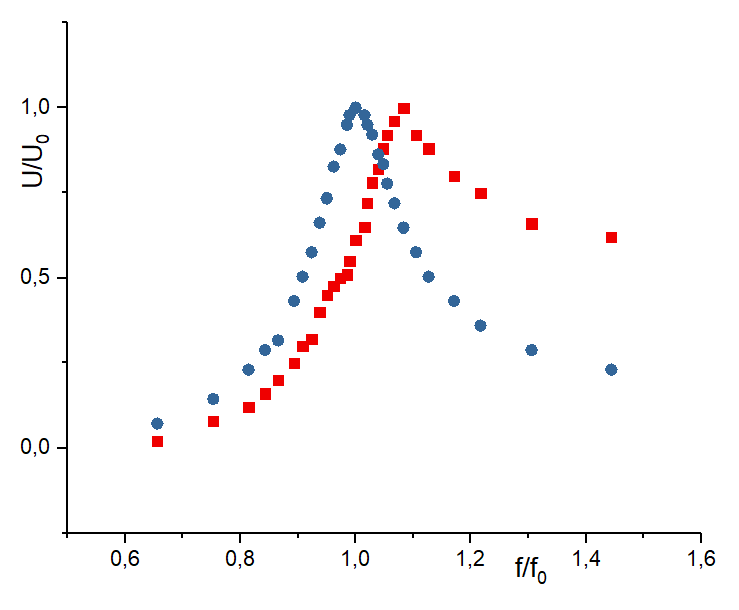
\includegraphics[width=0.55\linewidth]{1}
\end{figure}
Определим добротность по формуле $Q = \frac{\omega_0}{2\Delta\Omega}$ 
\\
Получим: $\boxed {Q_{R=0} = 36,364; \ \  Q_{R=100} = 7,407}$ \\\\
\textbf{2)} Устанавливаем в режиме цуг резонансную частоту генератора. Измеряем на экране осциллографа амплитуды двух колебаний $U_k$ и $U_{k+n}$ в режиме нарастания колебаний, разделённых целым числом $n$ периодов, и амплитуду установившихся колебаний $U_0$ при $R=0$ и $R=100$ Ом. Вычисляем добротность
$$
Q=\frac{\pi n}{\ln\frac{U_0-U_k}{U_0-U_{k+n}}},\ 
\sigma_Q=\frac{Q^2}{\pi n}\sqrt{\frac{2\sigma_U^2}{(U_0-U_k)^2}+\frac{2\sigma_U^2}{(U_0-U_{k+n})^2}}
$$
Результаты измерений и вычислений в таб.~3.
\begin{table}[h!]
	\begin{center}
			\textbf{Таблица 3}.\\
		\begin{tabular}{|c|c|c|c|c||c|c|c|c|c|}
			\hline\multicolumn{5}{|c||}{$R=0$}&\multicolumn{5}{c|}{$R=100$ Ом}\\
			\hhline{|-|-|-|-|-||-|-|-|-|-|}
			$U_k$, дел&$U_{k+n}$, дел&$n$&$U_0$, дел&$Q$&
			$U_k$, дел&$U_{k+n}$, дел&$n$&$U_0$, дел&$Q$\\
			\hhline{|-|-|-|-|-||-|-|-|-|-|}
			1,2&2,2&6&\multirow{4}{*}{7,0}&$27\pm5$
			&1,2&3,8&6&\multirow{4}{*}{4,0}&$7\pm4$
			\\
			\hhline{|-|-|-|~|-||-|-|-|~|-|}
			3,0&6,0&11&&$25\pm5$&1,8&3,8&5&&$7\pm4$\\
			\hhline{|-|-|-|~|-||-|-|-|~|-|}
			4,2&6,0&8&&$24\pm7$&2,2&3,8&4&&$6\pm4$\\
			\hhline{|-|-|-|~|-||-|-|-|~|-|}
			1,2&5,0&9&&$26\pm4$&2,4&3,8&3&&$5\pm3$\\
			\hline
			\multicolumn{10}{c}{\strut}\\
		\end{tabular}
	\end{center}
\end{table}\\
\textbf{3)} Измеряем на экране осциллографа амплитуды двух колебаний $U_k$ и $U_{k+n}$ в режиме затухания. Вычисляем добротность
$$
Q=\frac{\pi n}{\ln\frac{U_k}{U_{k+n}}},\ 
\sigma_Q=\frac{Q^2}{\pi n}\sqrt{\frac{\sigma_U^2}{U_k^2}+\frac{\sigma_U^2}{U_{k+n}^2}}
$$

Результаты измерений и вычислений в таб.~4.

\begin{table}[h!]
	\begin{center}
			\textbf{Таблица 4}.\\
		\begin{tabular}{|c|c|c|c||c|c|c|c|}
			\hline\multicolumn{4}{|c||}{$R=0$}&\multicolumn{4}{c|}{$R=100$ Ом}\\
			\hhline{|-|-|-|-||-|-|-|-|}
			$U_k$, дел&$U_{k+n}$, дел&$n$&$Q$&
			$U_k$, дел&$U_{k+n}$, дел&$n$&$Q$\\
			\hhline{|-|-|-|-||-|-|-|-|}	6	&	1	&	17	& $30\pm4$	&	3,2	&	2	&	1	&$7\pm2$\\
			\hhline{|-|-|-|-||-|-|-|-|}	5,4	&	1	&	16	&$30\pm4$	&	3,2	&	1,4	&	2	&$7,6\pm1,4$\\
			\hhline{|-|-|-|-||-|-|-|-|}	3,2	&	1	&	11	&$30\pm5$	&	3,2	&	1	&	3	&$8\pm2$\\
			\hhline{|-|-|-|-||-|-|-|-|}	2,4	&	1	&	8	&$29\pm7$	&	3,2	&	0,6	&	4	&$8\pm2$\\
			\hline
			\multicolumn{8}{c}{\strut}\\
			
		\end{tabular}
	\end{center}
\end{table}
\textbf{4)} Вычисляем теоретическое значение добротности контура
	$$
	Q=\frac1{R+R_L}\sqrt{\frac LC},\ \sigma_Q=Q\sqrt{ \frac{\sigma_R^2+\sigma_{R_L}^2}{(R+R_L)^2}+\left( \frac{\sigma_L}L\right) ^2+\left( \frac{\sigma_C}C\right) ^2}
	$$
	Сводим в таб.~5 все полученные значения добротности.
	\begin{table}[h!]
		\begin{center}
						\textbf{Таблица 5}.\\
			\begin{tabular}{|c||c|c|c|c|}
				\hline
				$R$, Ом&$ Q_{\mbox{рез}} $&$\left\langle Q\right\rangle_{{\nearrow}} $&$\left\langle Q\right\rangle_{{\searrow}} $&$ Q_{\mbox{теор}}$\\
				\hline0&$36,36$&$26\pm3$&$30\pm3$&$32,7\pm0,3$\\
				\hline100&$7,41$&$6\pm2$&$7,7\pm1,0$&$7,65\pm0,07$\\
				\hline
				\multicolumn{5}{c}{\strut}\\

			\end{tabular}
		\end{center}
	\end{table}
\end{document}